\documentclass{article}
\usepackage{fancyhdr}
\usepackage{graphicx}
\usepackage{hyperref}
\usepackage[a4paper, hmargin = 1.5cm, head = 4cm, bottom = 2cm]{geometry}

\pagestyle{fancy}
\lhead{\includegraphics[width=0.27\textwidth]{assets/eth_logo.pdf}}
\rhead{Computer Networks}
\lfoot{Spring Semester 2023}
\rfoot{\thepage}
\cfoot{}
\renewcommand{\footrulewidth}{1pt}

\begin{document}

\begin{titlepage}
    \thispagestyle{fancy}
    \renewcommand{\headrulewidth}{1pt}

    \center
    \vspace*{1.0cm}
    \Large Computer Networks \\[.5 cm]
    \large
    \normalsize
    Gnkgo, Informatik B. Sc. 4. Semester \\
    \vfill
\end{titlepage}

% Table of Contents
\tableofcontents
\newpage % Start content on a new page

\section{Internet}

\begin{itemize}
    \item Internet connects End Systems/ Hosts by a system of communications links and package switches
    \item Packets: data segment and header
    \item IP (Internet Protocol): Specifies the format for packets sent among routers and end systems
    \begin{itemize}
        \item unreliable service
        \item best-effort delivery
        \item modify before forwarding the packet to the next hop
        \begin{itemize}
            \item destination MAC address
            \item Time-to-live
            \item IP checksum
        \end{itemize}
    \end{itemize}
    \item DSL (digital subscriber line): broadband residential access
    \begin{itemize}
        \item downstream data channel: tens to few hundred Mbps
        \item upstream data channel: few Mbps to few tens Mbps
    \end{itemize}
    \item FDM (Frequency-division multiplexing): link dedicates a frequency band on the band to a communication for the duration of connection. The width of this band is called bandwidth.
    \item TDM (time-division multiplexing): time is divided into frames of fixes size, and each frame is split into a fixed amount of slots. These slots are dedicated to one connection
\end{itemize}

\section{Packet, Circuit Switching}

\begin{itemize}
    \item Packet switching relies on buffers to account for unexpected bursts
    \item Circuit switching is better applicable when the peak-to-average utilization ratio is low.
    \item large Peak / Average $\rightarrow$ On-demand
    \item small peak /average $\rightarrow$ circuit
\end{itemize}

\section{Delays}

\begin{itemize}
    \item \textbf{nodal processing delay:}
    \begin{itemize}
        \item Time used to decode the header, determine which output needs to be used, bit-level checking, etc.
        \item Negligible in comparison to other delays, little room for improvement here
    \end{itemize}
    \item \textbf{queuing delay:}
    \begin{itemize}
        \item Time that the packet has to wait in the queue until the desired output will be free
        \item Better load balancing (i.e., via routing), reduce queue size
    \end{itemize}
    \item \textbf{transmission delay:}
    \begin{itemize}
        \item Time after the packet gets out of the queue until it's on the output line; let $L$ be the length of the packet, $R$ the transmission rate from router A to B, then the transmission delay is $L/R$.
        \item Increase the link capacity
    \end{itemize}
    \item \textbf{propagation delay:}
    \begin{itemize}
        \item Time the package takes to propagate through the physical medium (e.g., at light speed with radio waves), i.e., it takes on the way from router A to B
        \item If possible, use data replication to shorten the client-server distance. Improving routing or physical transmission media also helps
    \end{itemize}
\end{itemize}

\section{Layers}

\begin{center}
    \begin{tabular}{|c|}
        \hline
        Layers \\
        \hline
        Application \\
        \hline
        Transport \\
        \hline
        Network \\
        \hline
        Link \\
        \hline
        Physical \\
        \hline
    \end{tabular}
\end{center}

\begin{itemize}
    \item \textbf{Application Layer:} Application protocols and layers reside here. The internet includes many protocols here, as HTTP (provides Web document requests and responses), SMTP (for e-mail transfer), and FTP (file transfer from host to host). The DNS is also an application layer protocol. Packet of information at this layer is called a message.
    \item \textbf{Transport Layer:} Transports application layer messages between application endpoints. In the internet, there’s TCP and UDP. E.g. longer messages are split into shorter segments. Packets in this layer are called segments (TCP \& UDP) or Datagram (UDP).
    \item \textbf{Network Layer:} The layer is responsible for moving datagrams from host to host. It receives a segment and an address. This layer includes the IP, which defines the fields in a datagram and how to work on those fields. Packets in this layer are called datagrams / packet.
    \begin{itemize}
        \item ARP: broadcast domain receives everyone until a router.
        \item Goes through MAC.
    \end{itemize}
    \item \textbf{Link Layer:} The network layer brings a datagram from one node to another, but to move a packet from one specific node to another, it relies on the link layer.
    \begin{itemize}
        \item It delivers the packet to the next node. E.g. Ethernet or WiFi. Link layer protocols are called frames.
        \item Error detection
    \end{itemize}
    \item An Ethernet switch can interconnect a 10 Mbps Ethernet network and a 1 Gbps Ethernet network.
    \item The 802.11b wireless protocol incorporates a link-layer ACK not present in regular Ethernet.
    \item \textbf{Physical layer:} The job of the link layer is to move whole frames from one node to another; however, the job of the physical layer is to move individual bits. Many protocols exist, depending on the physical medium; e.g. Ethernet has different protocols for different cable types.
\end{itemize}

\section{Address Resolution Protocol (ARP)}

\begin{itemize}
    \item It allows a host to get the MAC address associated with an IP address.
\end{itemize}

\section{Ethernet}

\begin{enumerate}
    \item Frame starts with destination address.
    \begin{itemize}
        \item If not destined to this device, it can be simply dropped.
    \end{itemize}
    \item Source address.
    \item Type / length field.
    \begin{itemize}
        \item Tells receiver what payload this frame carries.
    \end{itemize}
    \item Data and pad.
    \begin{itemize}
        \item Minimum length of an Ethernet frame is 64 bytes in total.
    \end{itemize}
    \item Frame check sequence.
    \begin{itemize}
        \item Cyclic Redundancy Check (CRC) for error checking.
    \end{itemize}
\end{enumerate}

\section{Wireless Local Area Networks (WLANs)}

\begin{itemize}
    \item Multiple access points can operate on different channels.
    \item Nodes are often mobile, requiring dynamic routing.
\end{itemize}

\section{TCP/IP Model}

\begin{center}
    \begin{tabular}{|c|}
        \hline
        TCP/IP Model \\
        \hline
        Application Layer \\
        \hline
        Transport Layer \\
        \hline
        Internet Layer \\
        \hline
        Network Interface Layer \\
        \hline
    \end{tabular}
\end{center}

\begin{itemize}
    \item The network interface layer encompasses both the link and physical layers.
\end{itemize}

\section{Congestion Control}

\begin{itemize}
    \item A state in which one link in a subnet is so overwhelmed that it cannot effectively handle the amount of traffic that could use it.
    \item A link can become congested even if it has sufficient bandwidth.
    \item Network layer congestion can occur even if no link is congested.
\end{itemize}



\subsection{Receive Procedure}
\begin{enumerate}
    \item Divide and check for zero remainder
\end{enumerate}

\subsection{Path Lookup}
\begin{figure}[h]
    \centering
    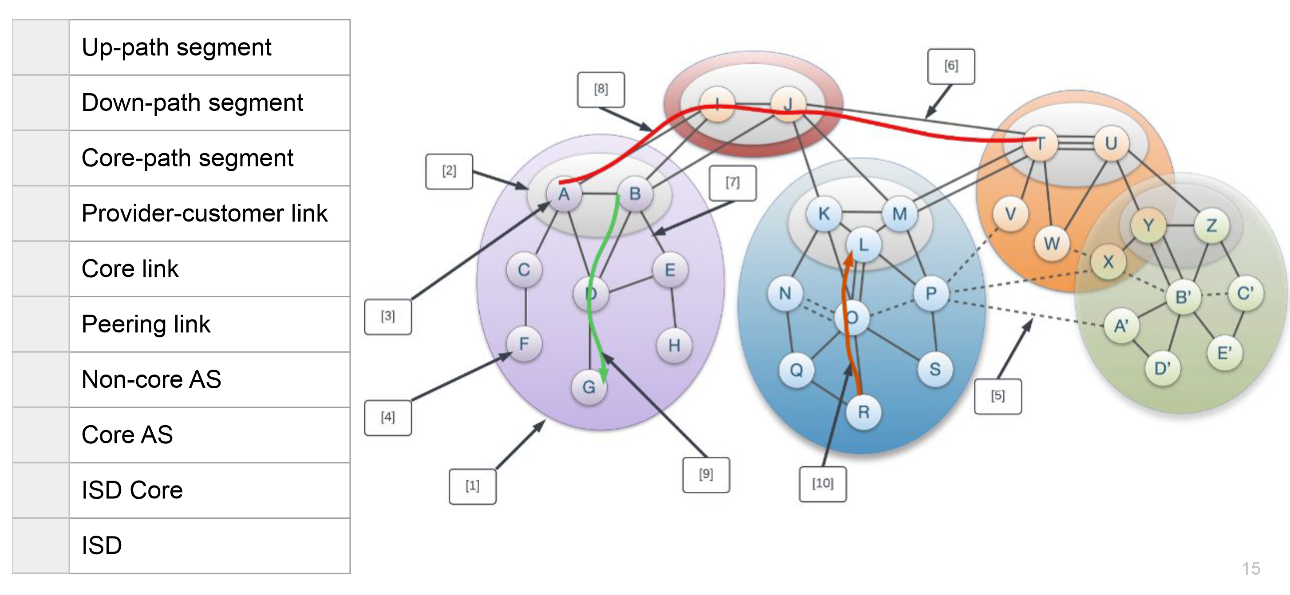
\includegraphics[width=0.8\textwidth]{assets/internet.png}
    \caption{Path Lookup}
\end{figure}

\subsection{Recipe to get IP addressing:}
\begin{table}[h]
    \centering
    \begin{tabular}{|c|p{10cm}|}
        \hline
        \textbf{Column Name} & \textbf{Explanation} \\
        \hline
        Prefix & The prefix notation (CIDR) representing the subnet's network size. IP address followed by a slash and the number of significant bits in the subnet mask. \\
        \hline
        \# of hosts & Maximum number of usable hosts in the subnet. Calculated as $2^{(32 - \mathrm{prefix length})} - 2$, accounting for network and broadcast addresses. \\
        \hline
        Prefix mask & Subnet mask in dotted-decimal notation, each segment represents 8 bits. \\
        \hline
        Network Address & Obtained by bitwise AND operation between IP address and subnet mask. \\
        \hline
        Broadcast Address & Highest address in the subnet, obtained by flipping all host bits to 1s in the network address. \\
        \hline
        Last Host Address & Highest usable IP address, obtained by setting all host bits to 1s in the network address, except for the last bit. \\
        \hline
    \end{tabular}
    \caption{IP Addressing Recipe}
\end{table}

\begin{figure}[h]
    \centering
    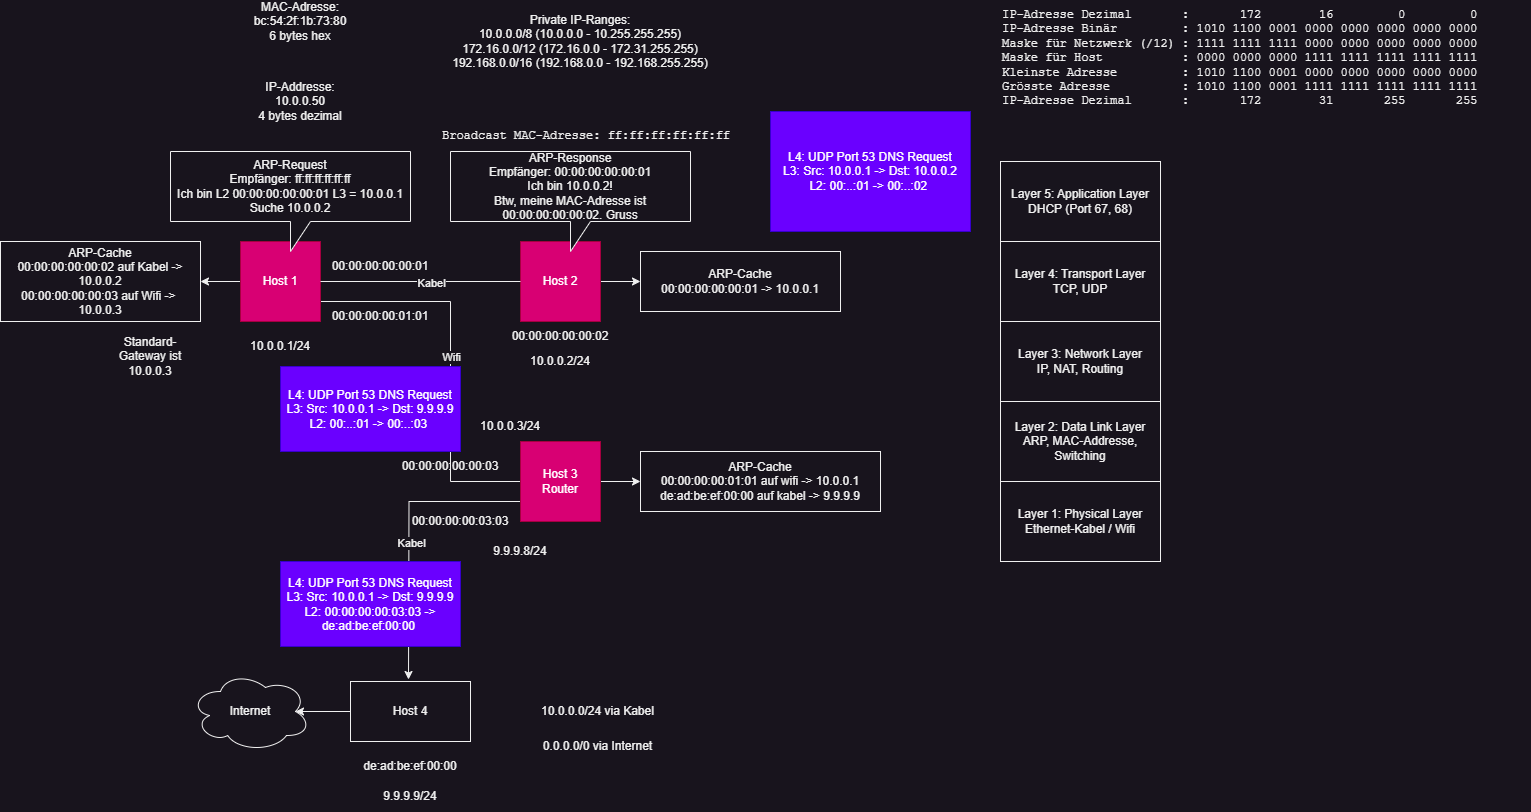
\includegraphics[width=0.8\textwidth]{assets/MAC_vs_IP-ARP+Routing.drawio.png}
    \caption{Mac vs IP-Address}
\end{figure}

\section{Quiz}
\begin{itemize}
    \item \textbf{The Maximum Segment Size (MSS) of TCP is equal to:}
    MSS = MTU - header(IP) - header(TCP)
    \item UDP sockets type is SOCK\_DGRAM while TCP sockets type is SOCK\_STREAM.
    \item For a SOCK\_STREAM, an operating system stores both local and remote port.
    \item Given a directed graph G(V, E), with \(|V|\) and \(|E|\) being the numbers of vertices and edges, how many variables do you need for the max-flow LP formulation discussed in class?
    \item There is no connection establishment in UDP.
    \item The objective of flow control is not to overwhelm the hosts.
    \item The objective of congestion control is to not overwhelm the network.
    \item During congestion avoidance in TCP, the successful acknowledgment of a segment results in the sender congestion window growing by one segment per RTT.
    \item TCP (SOCK\_STREAM) is a connection-based protocol. The connection is established, and the two parties have a conversation until the connection is terminated by one of the parties or by a network error.
    \item UDP (SOCK\_DGRAM) is a datagram-based protocol. You send one datagram and get one reply, and then the connection terminates.
    \item Given a directed graph G(V, E), with \(|V|\) and \(|E|\) being the numbers of vertices and edges, how many variables do you need for the max-flow LP formulation discussed in class?: \(O(|E|)\)
    \item QUIC can handle switching from WiFi to a cellular network without having to reestablish the connection:
    \begin{itemize}
        \item Uses connection IDs independent of the IP address instead of a 4-tuple like TCP to identify connections.
        \item This way packets using the connection ID are still valid, even if the source IP address changes.
    \end{itemize}
    \item If we create our simple query (\texttt{dig @a.root-servers.net www.ethz.ch}) and send it to the first root-server, we don’t get a \texttt{www.ethz.ch} IP in return. Why is this?
    \begin{itemize}
        \item Root server does not support recursive resolution.
    \end{itemize}
    \item The minimum information one needs to resolve any DNS hostname is the IP address of a DNS root server.
\end{itemize}

\section{Quic}
\begin{itemize}
    \item Operate in Application and Transport layer.
    \item Combines connection and TLS handshake $\rightarrow$ reducing the connection setup time by one RTT.
    \item Enables Zero-RTT communication if the hosts have communicated before (improved handshake).
    \item Connection hand-over is possible by identifying connection with a connection ID instead of the 5(/4)-tuple (even with changing IP addresses e.g. when changing networks with a mobile device).
    \item Resolves head-of-line blocking by the logical abstraction of streams (contrary to TCP, which required you to open multiple parallel TCP connections).
    \item Middleboxes and NAT routers are known to drop unfamiliar transport layer protocols. Quic uses UDP to give inseparability with existing hardware.
\end{itemize}

\end{document}
